% Beamer Final Presentation — Multimodal Sentiment Analysis
% Compile: pdflatex presentation.tex  (run twice for references)

\documentclass[aspectratio=169,10pt]{beamer}

% ---- Theme ----
\usetheme{metropolis}
\usecolortheme{default}
\setbeamertemplate{navigation symbols}{}
\setbeamertemplate{footline}[frame number]
\setbeamerfont{footnote}{size=\tiny}

% ---- Packages ----
\usepackage[utf8]{inputenc}
\usepackage[T1]{fontenc}
\usepackage{amsmath, amssymb}
\usepackage{booktabs}
\usepackage{multirow}
\usepackage{array}
\usepackage{colortbl}
\usepackage{graphicx}
\usepackage{xcolor}
\usepackage{tikz}
\usetikzlibrary{positioning, arrows.meta, calc, shapes, shapes.geometric, fit, backgrounds, matrix}
\usepackage{pgfplots}
\pgfplotsset{compat=1.18}
\usepgfplotslibrary{colorbrewer}

% ---- Colors ----
\definecolor{tblue}{RGB}{31,119,180}
\definecolor{torange}{RGB}{255,127,14}
\definecolor{tgreen}{RGB}{44,160,44}
\definecolor{tred}{RGB}{214,39,40}
\definecolor{tpurple}{RGB}{148,103,189}
\definecolor{tteal}{RGB}{23,190,207}
\definecolor{darkblue}{RGB}{0,70,140}
\definecolor{lightgray}{RGB}{230,230,230}

% ---- Metropolis tweaks ----
\setbeamercolor{progress bar}{fg=darkblue}
\setbeamercolor{frametitle}{fg=white,bg=darkblue}

% ---- Compact items ----
\setlength{\leftmargini}{1em}
\setbeamertemplate{itemize item}{\color{darkblue}$\bullet$}
\setbeamertemplate{itemize subitem}{\color{darkblue}$\circ$}

% ---- Title ----
\title{Multimodal Sentiment and Emotion Analysis}
\subtitle{Multi-Layer Feature Fusion and Multi-Task Learning}
\author{Manas Inamdar \and Soham Jahagirdar \and Parth Tokekar \and Gautam Gandhi}
\institute{Team TokeNization \\ Introduction to NLP (S26) --- Final Submission}
\date{April 2026}

% ============================================================
\begin{document}

% ---- Title slide ----
\begin{frame}
  \titlepage
\end{frame}

% ---- Outline ----
\begin{frame}{Outline}
  \begin{columns}[t]
    \column{0.5\textwidth}
    \begin{enumerate}
      \item Motivation \& Problem
      \item Related Work
      \item Datasets
      \item UFEN Architecture
      \item MTFN Architecture
      \item Multi-Task Loss
    \end{enumerate}
    \column{0.5\textwidth}
    \begin{enumerate}
      \setcounter{enumi}{6}
      \item Phase 1: CMU-MOSI Results
      \item Phase 2: MELD Experiment Trail
      \item Best Result (Exp 9.1)
      \item Analysis \& Ablations
      \item Limitations \& Future Work
      \item Conclusion
    \end{enumerate}
  \end{columns}
  \vfill
  \centering\small
  \textbf{Paper re-implemented:} Cai et al., \emph{Sci.\ Reports} 2025 (UFEN+MTFN).
\end{frame}

% ============================================================
\section{Motivation}
% ============================================================

\begin{frame}{Why Multimodal?}
  \begin{columns}[c]
    \column{0.55\textwidth}
    Human communication is multimodal:
    \begin{itemize}
      \item \textbf{Text} --- what is said
      \item \textbf{Audio} --- how it is said
      \item \textbf{Video} --- facial reaction
    \end{itemize}
    \vspace{0.4em}
    \emph{``It was fine.''} \\[0.3em]
    \small
    \begin{tabular}{ll}
      Text only & $\to$ neutral \\
      + flat voice & $\to$ negative \\
      + frown     & $\to$ disappointed
    \end{tabular}

    \column{0.45\textwidth}
    \centering
    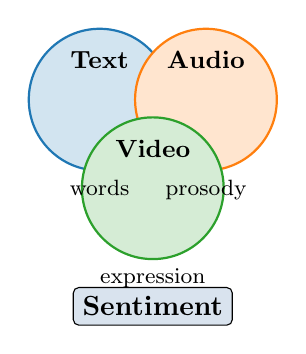
\begin{tikzpicture}[scale=0.75, every node/.style={font=\small}]
      % Modality circles
      \draw[fill=tblue!20, draw=tblue, thick] (0,0) circle (1.2) node[yshift=0.5cm]{\textbf{Text}};
      \draw[fill=torange!20, draw=torange, thick] (1.8,0) circle (1.2) node[yshift=0.5cm]{\textbf{Audio}};
      \draw[fill=tgreen!20, draw=tgreen, thick] (0.9,-1.5) circle (1.2) node[yshift=0.5cm]{\textbf{Video}};
      \node[below, font=\footnotesize] at (0,-1.2) {words};
      \node[below, font=\footnotesize] at (1.8,-1.2) {prosody};
      \node[below, font=\footnotesize] at (0.9,-2.7) {expression};
      \node[draw, fill=darkblue!15, rounded corners=2pt, font=\bfseries] at (0.9,-3.5) {Sentiment};
    \end{tikzpicture}
  \end{columns}
\end{frame}

\begin{frame}{Three Core Challenges}
  \centering
  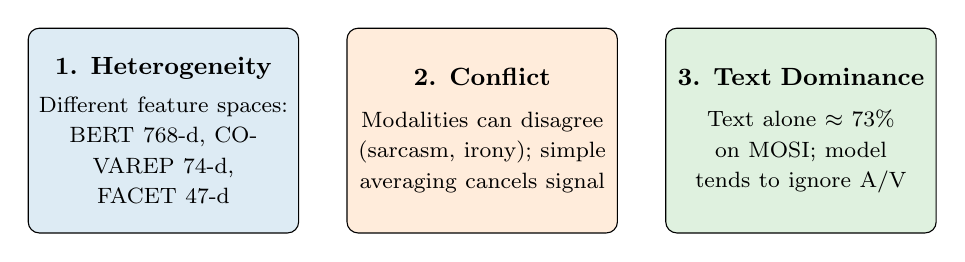
\begin{tikzpicture}[every node/.style={font=\small}, node distance=0.6cm]
    \node[draw, rounded corners, fill=tblue!15, minimum width=3.4cm, minimum height=2.6cm, text width=3.2cm, align=center]
      (c1) {\textbf{1. Heterogeneity}\\[4pt]\footnotesize Different feature spaces:\\BERT 768-d, COVAREP 74-d, FACET 47-d};
    \node[draw, rounded corners, fill=torange!15, minimum width=3.4cm, minimum height=2.6cm, text width=3.2cm, align=center, right=of c1]
      (c2) {\textbf{2. Conflict}\\[4pt]\footnotesize Modalities can disagree (sarcasm, irony); simple averaging cancels signal};
    \node[draw, rounded corners, fill=tgreen!15, minimum width=3.4cm, minimum height=2.6cm, text width=3.2cm, align=center, right=of c2]
      (c3) {\textbf{3. Text Dominance}\\[4pt]\footnotesize Text alone $\approx$ 73\% on MOSI; model tends to ignore A/V};
  \end{tikzpicture}
  \vfill
  \textbf{UFEN+MTFN} addresses all three with a two-stage pipeline
  and five-task supervision.
\end{frame}

% ============================================================
\section{Related Work \& Datasets}
% ============================================================

\begin{frame}{Related Work}
  \small
  \begin{tabular}{ll}
    \toprule
    \textbf{Category} & \textbf{Representative Methods} \\
    \midrule
    Per-modality encoders & BERT, LSTM/GRU, COVAREP, FACET \\
    Tensor fusion         & TFN, LMF \\
    Attention fusion      & MulT, MFN, MISA \\
    Multi-task MSA        & Self-MM, MMIM \\
    ERC on MELD           & DialogueRNN, DialogueGCN, MM-DFN, MultiEMO \\
    \midrule
    \textbf{Our base paper} & \textbf{UFEN+MTFN} (Cai et al., 2025) \\
    \bottomrule
  \end{tabular}
  \vspace{0.7em}

  UFEN+MTFN combines MulT-style cross-modal attention with Self-MM-style
  multi-task learning and adds a Transformer encoder--decoder on top.
\end{frame}

\begin{frame}{Datasets}
  \begin{columns}[t]
    \column{0.5\textwidth}
    \textbf{CMU-MOSI} (Phase 1)
    \begin{itemize}
      \item 2{,}199 YouTube review clips
      \item Regression: $[-3, +3]$
      \item Splits: 1{,}283 / 214 / 686
      \item Text: BERT-768 (fine-tuned)
      \item Audio: COVAREP 74-d
      \item Visual: FACET 47-d
    \end{itemize}

    \column{0.5\textwidth}
    \textbf{MELD} (Phase 2)
    \begin{itemize}
      \item 13{,}708 \emph{Friends} utterances
      \item 7-class classification
      \item Splits: 9{,}988 / 1{,}108 / 2{,}610
      \item Strongly imbalanced
    \end{itemize}
  \end{columns}
  \vspace{0.5em}
  \centering
  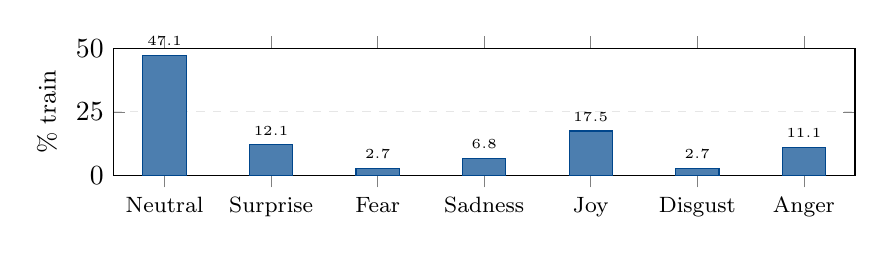
\begin{tikzpicture}
    \begin{axis}[
      width=11cm, height=3.2cm,
      ybar, bar width=0.55cm,
      ymin=0, ymax=50,
      ylabel={\small \% train},
      symbolic x coords={Neutral,Surprise,Fear,Sadness,Joy,Disgust,Anger},
      xtick=data, x tick label style={font=\footnotesize, rotate=0},
      ytick={0,25,50}, ytick style={font=\footnotesize},
      ymajorgrids, grid style={dashed, lightgray},
      nodes near coords, nodes near coords style={font=\tiny},
      enlarge x limits=0.08,
    ]
      \addplot[fill=darkblue!70, draw=darkblue] coordinates {
        (Neutral,47.1) (Surprise,12.1) (Fear,2.7) (Sadness,6.8)
        (Joy,17.5) (Disgust,2.7) (Anger,11.1)
      };
    \end{axis}
  \end{tikzpicture}
  \centering\footnotesize MELD label distribution (train split).
\end{frame}

% ============================================================
\section{Architecture}
% ============================================================

\begin{frame}{Architecture Overview}
  \centering
  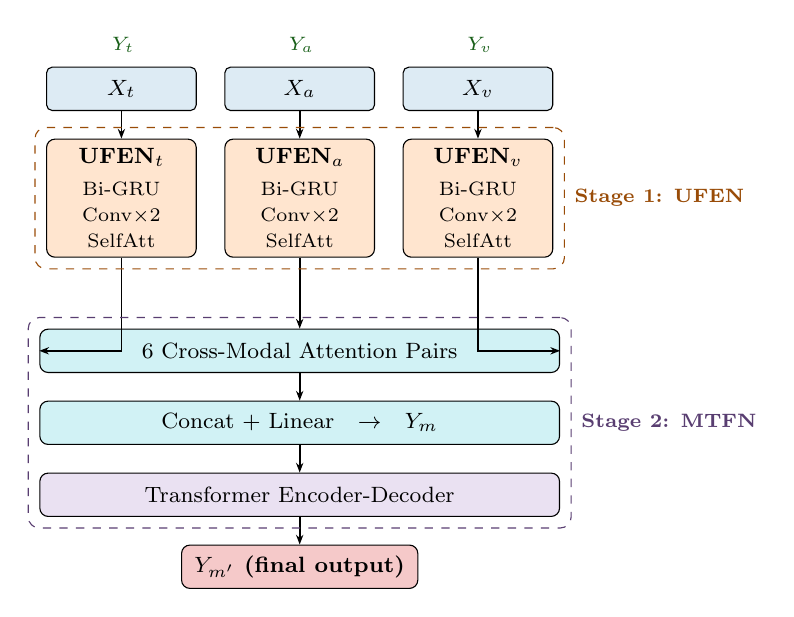
\begin{tikzpicture}[
      every node/.style={font=\footnotesize},
      node distance=0.35cm and 0.35cm,
      inp/.style={draw, rounded corners=2pt, fill=tblue!15, minimum width=1.9cm, minimum height=0.55cm, align=center},
      ufen/.style={draw, rounded corners=3pt, fill=torange!20, minimum width=1.9cm, minimum height=1.2cm, align=center},
      wide/.style={draw, rounded corners=3pt, fill=tteal!20, minimum width=6.6cm, minimum height=0.55cm, align=center},
      mfuse/.style={draw, rounded corners=3pt, fill=tpurple!20, minimum width=6.6cm, minimum height=0.55cm, align=center},
      finaln/.style={draw, rounded corners=3pt, fill=tred!25, minimum width=3cm, minimum height=0.55cm, align=center, font=\footnotesize\bfseries},
      arr/.style={-{Stealth[length=3.5pt]}, semithick},
  ]
    \node[inp] (xt) {$X_t$};
    \node[inp, right=of xt] (xa) {$X_a$};
    \node[inp, right=of xa] (xv) {$X_v$};

    \node[ufen, below=of xt] (ut) {\textbf{UFEN}$_t$\\[2pt]\scriptsize Bi-GRU\\\scriptsize Conv$\times$2\\\scriptsize SelfAtt};
    \node[ufen, below=of xa] (ua) {\textbf{UFEN}$_a$\\[2pt]\scriptsize Bi-GRU\\\scriptsize Conv$\times$2\\\scriptsize SelfAtt};
    \node[ufen, below=of xv] (uv) {\textbf{UFEN}$_v$\\[2pt]\scriptsize Bi-GRU\\\scriptsize Conv$\times$2\\\scriptsize SelfAtt};

    \draw[arr](xt)--(ut);
    \draw[arr](xa)--(ua);
    \draw[arr](xv)--(uv);

    \node[above=0.05cm of xt, font=\scriptsize, tgreen!60!black] {\,$Y_t$};
    \node[above=0.05cm of xa, font=\scriptsize, tgreen!60!black] {\,$Y_a$};
    \node[above=0.05cm of xv, font=\scriptsize, tgreen!60!black] {\,$Y_v$};

    \node[wide, below=0.9cm of ua] (ca) {6 Cross-Modal Attention Pairs};
    \draw[arr](ut.south) |- (ca);
    \draw[arr](ua.south)  -- (ca);
    \draw[arr](uv.south) |- (ca);

    \node[wide, below=of ca] (concat) {Concat $+$ Linear\quad$\to$\quad$Y_m$};
    \draw[arr](ca)--(concat);

    \node[mfuse, below=of concat] (ed) {Transformer Encoder-Decoder};
    \draw[arr](concat)--(ed);

    \node[finaln, below=of ed] (ym) {$Y_{m'}$ (final output)};
    \draw[arr](ed)--(ym);

    \node[draw=torange!60!black, dashed, rounded corners, fit=(ut)(uv), inner sep=4pt, label=right:{\scriptsize \textcolor{torange!60!black}{\textbf{Stage 1: UFEN}}}] {};
    \node[draw=tpurple!60!black, dashed, rounded corners, fit=(ca)(concat)(ed), inner sep=4pt, label=right:{\scriptsize \textcolor{tpurple!60!black}{\textbf{Stage 2: MTFN}}}] {};
  \end{tikzpicture}
\end{frame}

\begin{frame}{Stage 1: UFEN --- Unimodal Feature Extraction}
  \begin{columns}[T]
    \column{0.52\textwidth}
    \small
    One UFEN per modality. Five steps:
    \vspace{0.3em}
    \begin{enumerate}
      \item \textbf{Bi-GRU} captures temporal context in both directions
      \item \textbf{Parallel Conv1D} branches (kernels $[1, 5]$) extract multi-scale patterns
      \item \textbf{Self-attention gate}:\\ $X \otimes \text{Att}(X)$ amplifies salient steps
      \item \textbf{Unpool $+$ sum} across branches
      \item \textbf{Unimodal head} $\to Y_i$\\ (used in multi-task loss)
    \end{enumerate}

    \column{0.48\textwidth}
    \centering
    \vspace{0.2em}
    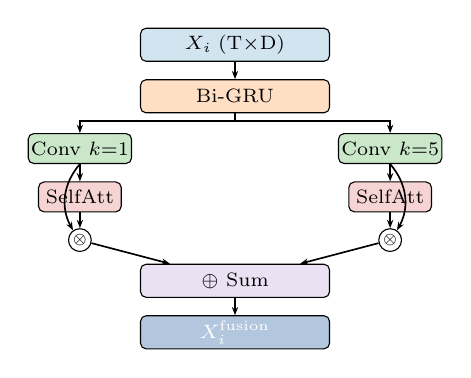
\begin{tikzpicture}[every node/.style={font=\scriptsize},
        block/.style={draw, rounded corners=2pt, minimum width=2.4cm, minimum height=0.42cm, align=center, inner sep=1pt},
        smallblock/.style={draw, rounded corners=2pt, minimum width=1.05cm, minimum height=0.38cm, align=center, inner sep=1pt},
        arr/.style={-{Stealth[length=3pt]}, semithick},
        node distance=0.22cm]
      \node[block, fill=tblue!20] (input) {$X_i$\;(T$\times$D)};
      \node[block, fill=torange!25, below=of input] (gru) {Bi-GRU};
      \node[smallblock, fill=tgreen!25, below left=0.25cm and 0.1cm of gru] (c1) {Conv $k{=}1$};
      \node[smallblock, fill=tgreen!25, below right=0.25cm and 0.1cm of gru] (c2) {Conv $k{=}5$};
      \node[smallblock, fill=tred!20, below=of c1] (a1) {SelfAtt};
      \node[smallblock, fill=tred!20, below=of c2] (a2) {SelfAtt};
      \node[draw, circle, inner sep=0.5pt, below=0.2cm of a1, fill=white, font=\tiny] (g1) {$\otimes$};
      \node[draw, circle, inner sep=0.5pt, below=0.2cm of a2, fill=white, font=\tiny] (g2) {$\otimes$};
      \node[block, fill=tpurple!20, below=0.3cm of gru |- g1] (add) {$\oplus$ Sum};
      \node[block, fill=darkblue!30, text=white, below=of add] (out) {$X_i^{\text{fusion}}$};

      \draw[arr](input)--(gru);
      \draw[arr](gru.south) -- ++(0,-0.1) -| (c1);
      \draw[arr](gru.south) -- ++(0,-0.1) -| (c2);
      \draw[arr](c1)--(a1);
      \draw[arr](c2)--(a2);
      \draw[arr](a1)--(g1);
      \draw[arr](a2)--(g2);
      \draw[arr](c1.south) to[bend right=35] (g1);
      \draw[arr](c2.south) to[bend left=35] (g2);
      \draw[arr](g1)--(add);
      \draw[arr](g2)--(add);
      \draw[arr](add)--(out);
    \end{tikzpicture}
  \end{columns}
\end{frame}

\begin{frame}{Stage 2: MTFN --- Multi-Task Fusion}
  \small
  \textbf{Six directed cross-modal attention pairs:}
  \vspace{-0.3em}
  \[
    \text{CA}_{i \to j} = \text{LN}\bigl(\text{MHAtt}(Q_i, K_j, V_j)\bigr),
    \quad (i,j) \in \{t,a,v\}^2,\ i \neq j
  \]

  \begin{columns}[c]
    \column{0.55\textwidth}
    \centering
    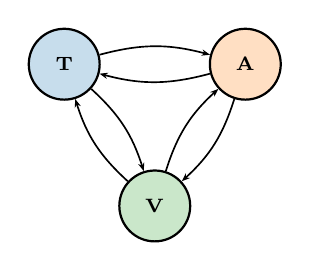
\begin{tikzpicture}[every node/.style={font=\scriptsize},
        mod/.style={draw, circle, minimum size=0.9cm, thick},
        arr/.style={-{Stealth[length=3pt]}, semithick}]
      \node[mod, fill=tblue!25] (t) at (0,0) {\textbf{T}};
      \node[mod, fill=torange!25] (a) at (2.3,0) {\textbf{A}};
      \node[mod, fill=tgreen!25] (v) at (1.15,-1.8) {\textbf{V}};

      \draw[arr, bend left=15] (t) to (a);
      \draw[arr, bend left=15] (a) to (t);
      \draw[arr, bend left=15] (t) to (v);
      \draw[arr, bend left=15] (v) to (t);
      \draw[arr, bend left=15] (a) to (v);
      \draw[arr, bend left=15] (v) to (a);
    \end{tikzpicture}

    \column{0.45\textwidth}
    \begin{itemize}
      \item Each pair $\to$ mean-pool
      \item Concat $6 \times d_m$ $\to Y_m$
      \item Reshape to length-6 seq
      \item Transformer enc--dec refines
      \item Final prediction $Y_{m'}$
    \end{itemize}
  \end{columns}
\end{frame}

\begin{frame}{Multi-Task Loss: 5 Heads, 1 Objective}
  \begin{equation*}
    \mathcal{L}_{\text{total}} = \underbrace{\mathcal{L}_t + \mathcal{L}_a + \mathcal{L}_v}_{\text{unimodal}}
    \;+\; \underbrace{\mathcal{L}_m + \mathcal{L}_{m'}}_{\text{multimodal}}
  \end{equation*}
  \vspace{0.3em}
  \begin{columns}[t]
    \column{0.5\textwidth}
    \textbf{Why 5 losses?}
    \begin{itemize}
      \item Without unimodal losses, model ignores A/V
      \item Text alone reaches $\sim$73\% on MOSI
      \item Forces each branch to carry signal
    \end{itemize}

    \column{0.5\textwidth}
    \textbf{Task-specific variants}
    \begin{itemize}
      \item Phase 1 (MOSI): MSE, 5 regression heads
      \item Phase 2 (MELD): Weighted cross-entropy + label smoothing, 5 classification heads
    \end{itemize}
  \end{columns}
  \vspace{0.7em}
  \centering
  \footnotesize\emph{Test-time output is $Y_{m'}$ only; the other four heads exist only during training.}
\end{frame}

% ============================================================
\section{Phase 1: CMU-MOSI}
% ============================================================

\begin{frame}{Phase 1: CMU-MOSI --- Best Configuration (P3-2)}
  \begin{columns}[t]
    \column{0.45\textwidth}
    \small
    \textbf{Search scope:} 25+ experiments in 3 sub-phases
    \begin{itemize}
      \item \textbf{1a:} Single-param sweeps
      \item \textbf{1b:} Combinations
      \item \textbf{1c:} Regularisation
    \end{itemize}
    \vspace{0.3em}
    \textbf{Key unlocks}
    \begin{itemize}
      \item $d_{\text{ff}} = 128$ (not $2{\times}d_m$)
      \item Kernels $[1, 5]$
      \item Cosine LR + early stop = 15
      \item BERT warmup (5 epochs linear)
      \item Weight decay was catastrophic
    \end{itemize}

    \column{0.55\textwidth}
    \centering\small
    \begin{tabular}{lcc}
      \toprule
      \textbf{Metric} & \textbf{Ours (P3-2)} & \textbf{Paper} \\
      \midrule
      MAE $\downarrow$            & \textbf{0.812} & 0.728 \\
      Corr $\uparrow$             & \textbf{0.745} & 0.792 \\
      Acc-7 $\uparrow$            & \textbf{43.0}  & 46.7 \\
      Acc-2 nn $\uparrow$         & \textbf{78.6}  & 85.2 \\
      Acc-2 np $\uparrow$         & \textbf{80.3}  & 86.6 \\
      F1 np $\uparrow$            & \textbf{80.4}  & 86.7 \\
      \bottomrule
    \end{tabular}
    \vspace{0.5em}

    \footnotesize\emph{Dev MAE reached 0.7434 --- within 0.015 of paper's target.}

    \vspace{0.3em}
    \footnotesize $\sim$110.8M params (BERT dominates).
  \end{columns}
\end{frame}

\begin{frame}{Phase 1 Ablation --- Every Component Matters}
  \centering
  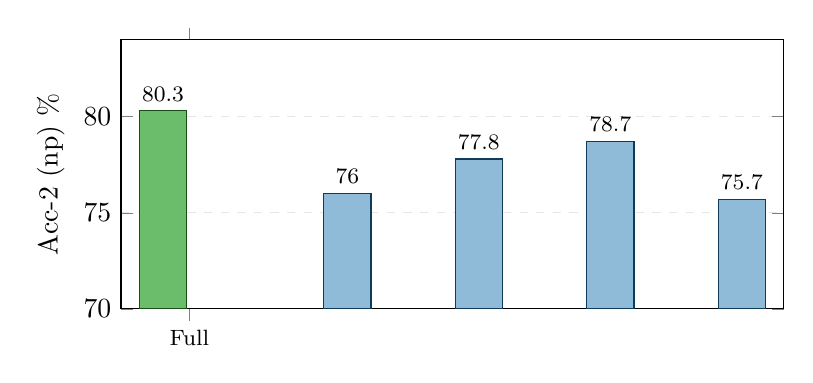
\begin{tikzpicture}
    \begin{axis}[
      width=10cm, height=5cm,
      ybar, bar width=0.6cm,
      ylabel={Acc-2 (np) \%},
      ymin=70, ymax=84,
      symbolic x coords={Full,No CA,No UniL,No ED,1 Conv},
      xtick=data, x tick label style={font=\footnotesize, align=center},
      ytick style={font=\footnotesize},
      ymajorgrids, grid style={dashed, lightgray},
      nodes near coords, nodes near coords style={font=\footnotesize},
      enlarge x limits=0.13,
    ]
      \addplot[fill=tgreen!70, draw=tgreen!50!black] coordinates {(Full,80.3)};
      \addplot[fill=tblue!50, draw=tblue!50!black] coordinates {(No CA,76.0) (No UniL,77.8) (No ED,78.7) (1 Conv,75.7)};
    \end{axis}
  \end{tikzpicture}
  \vfill
  \small
  \begin{itemize}
    \item \textbf{Cross-modal attention} $-4.3$ points $\to$ biggest component
    \item \textbf{Unimodal losses} $-2.5$ points $\to$ stop text collapse
    \item \textbf{Encoder--decoder} $-1.6$ points $\to$ refinement helps
    \item \textbf{Single conv} $-4.6$ points $\to$ multi-scale is essential
  \end{itemize}
\end{frame}

% ============================================================
\section{Phase 2: MELD}
% ============================================================

\begin{frame}{Phase 2 Experiment Trail --- Timeline}
  \centering
  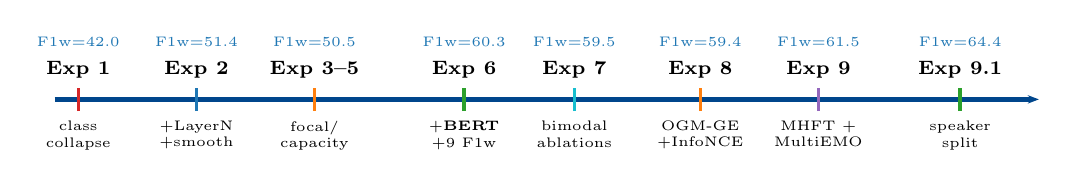
\begin{tikzpicture}[every node/.style={font=\scriptsize}]
    % Horizontal timeline
    \draw[-{Stealth[length=4pt]}, ultra thick, darkblue] (0,0) -- (12.5,0);

    % Experiment nodes (written out to avoid foreach tokenization issues)
    \draw[tred, very thick] (0.3,-0.15) -- (0.3,0.15);
    \node[above, font=\scriptsize\bfseries] at (0.3,0.15) {Exp 1};
    \draw[tblue, very thick] (1.8,-0.15) -- (1.8,0.15);
    \node[above, font=\scriptsize\bfseries] at (1.8,0.15) {Exp 2};
    \draw[torange, very thick] (3.3,-0.15) -- (3.3,0.15);
    \node[above, font=\scriptsize\bfseries] at (3.3,0.15) {Exp 3--5};
    \draw[tgreen, very thick] (5.2,-0.15) -- (5.2,0.15);
    \node[above, font=\scriptsize\bfseries] at (5.2,0.15) {Exp 6};
    \draw[tteal, very thick] (6.6,-0.15) -- (6.6,0.15);
    \node[above, font=\scriptsize\bfseries] at (6.6,0.15) {Exp 7};
    \draw[torange, very thick] (8.2,-0.15) -- (8.2,0.15);
    \node[above, font=\scriptsize\bfseries] at (8.2,0.15) {Exp 8};
    \draw[tpurple, very thick] (9.7,-0.15) -- (9.7,0.15);
    \node[above, font=\scriptsize\bfseries] at (9.7,0.15) {Exp 9};
    \draw[tgreen, very thick] (11.5,-0.15) -- (11.5,0.15);
    \node[above, font=\scriptsize\bfseries] at (11.5,0.15) {Exp 9.1};

    % Labels below
    \node[below, align=center, font=\tiny] at (0.3,-0.15) {class\\collapse};
    \node[below, align=center, font=\tiny] at (1.8,-0.15) {+LayerN\\+smooth};
    \node[below, align=center, font=\tiny] at (3.3,-0.15) {focal/\\capacity};
    \node[below, align=center, font=\tiny] at (5.2,-0.15) {+\textbf{BERT}\\+9 F1w};
    \node[below, align=center, font=\tiny] at (6.6,-0.15) {bimodal\\ablations};
    \node[below, align=center, font=\tiny] at (8.2,-0.15) {OGM-GE\\+InfoNCE};
    \node[below, align=center, font=\tiny] at (9.7,-0.15) {MHFT +\\MultiEMO};
    \node[below, align=center, font=\tiny] at (11.5,-0.15) {speaker\\split};

    % F1w annotations above
    \foreach \x/\val in {0.3/42.0, 1.8/51.4, 3.3/50.5, 5.2/60.3, 6.6/59.5, 8.2/59.4, 9.7/61.5, 11.5/64.4} {
      \node[above=0.55cm, font=\tiny, tblue] at (\x,0) {F1w=\val};
    }
  \end{tikzpicture}
  \vfill
  \small Three major jumps: Exp 2 (feature norm), Exp 6 (BERT), Exp 9.1 (MHFT + clean split).
\end{frame}

\begin{frame}{Phase 2 Results --- Weighted F1 Progression}
  \centering
  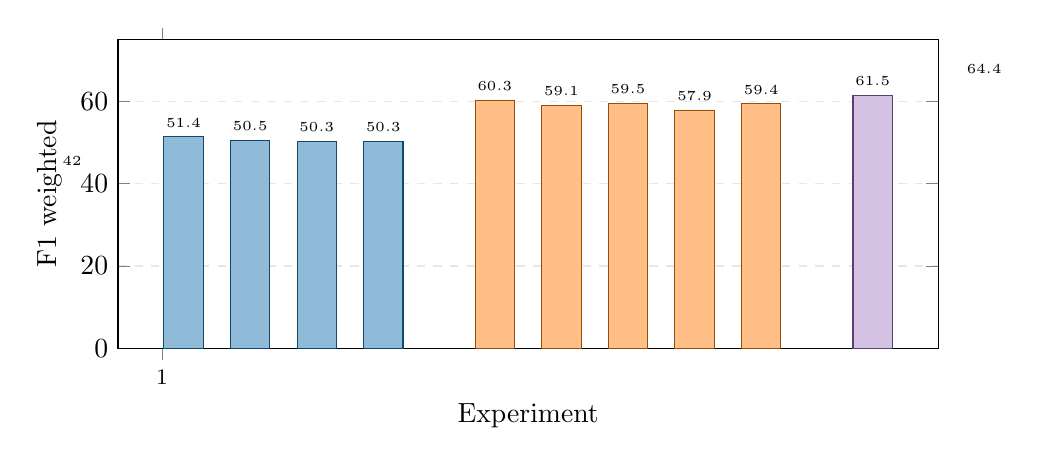
\begin{tikzpicture}
    \begin{axis}[
      width=12cm, height=5.5cm,
      ybar, bar width=0.5cm,
      ylabel={F1 weighted},
      ymin=0, ymax=75,
      symbolic x coords={1,2,3,4,5,6,7a,7b,7c,8,9,9.1},
      xtick=data, x tick label style={font=\footnotesize},
      xlabel={Experiment},
      ytick style={font=\footnotesize},
      ymajorgrids, grid style={dashed, lightgray},
      nodes near coords, nodes near coords style={font=\tiny},
      enlarge x limits=0.06,
    ]
      \addplot[fill=tred!50, draw=tred!60!black] coordinates {(1,42.0)};
      \addplot[fill=tblue!50, draw=tblue!60!black] coordinates {(2,51.4) (3,50.5) (4,50.3) (5,50.3)};
      \addplot[fill=torange!50, draw=torange!60!black] coordinates {(6,60.3) (7a,59.1) (7b,59.5) (7c,57.9) (8,59.4)};
      \addplot[fill=tpurple!40, draw=tpurple!60!black] coordinates {(9,61.5)};
      \addplot[fill=tgreen!70, draw=tgreen!50!black] coordinates {(9.1,64.4)};
    \end{axis}
  \end{tikzpicture}
  \vfill
  \footnotesize
  \textcolor{tred!70!black}{\textbf{Exp 1:}} collapse \quad
  \textcolor{tblue!70!black}{\textbf{2--5:}} GloVe plateau \quad
  \textcolor{torange!70!black}{\textbf{6--8:}} BERT (111M params) \quad
  \textcolor{tpurple!70!black}{\textbf{9:}} MHFT \quad
  \textcolor{tgreen!50!black}{\textbf{9.1:}} \textbf{best}
\end{frame}

\begin{frame}{Exp 1--2: Diagnosing Class Collapse}
  \begin{columns}[t]
    \column{0.5\textwidth}
    \textbf{Exp 1 failure:} only Neutral \& Anger predicted
    \vspace{0.3em}
    \small
    \begin{itemize}
      \item LR 5e-3 too high (oscillation)
      \item GloVe L2 norm $\approx$ 5 vs.\ audio 0.85, video 0.72 \\ $\to$ \textbf{7$\times$ text dominance}
      \item Trivial minimum: majority class only
    \end{itemize}

    \column{0.5\textwidth}
    \textbf{Exp 2 fix:} 3 targeted changes
    \vspace{0.3em}
    \small
    \begin{itemize}
      \item Per-modality LayerNorm
      \item LR $\to 10^{-3}$
      \item Label smoothing 0.1
    \end{itemize}
    \vspace{0.3em}
    \textbf{Result}
    \begin{itemize}
      \item F1w: $42.0 \to 51.4$ (\textbf{+9.4})
      \item F1m: $19.6 \to 33.1$ (\textbf{+13.5})
      \item All 7 classes get predictions
    \end{itemize}
  \end{columns}
\end{frame}

\begin{frame}{Exp 6: BERT Breaks the GloVe Ceiling}
  \begin{columns}[c]
    \column{0.5\textwidth}
    \small
    \textbf{Why GloVe plateaued:} context-free embeddings cannot disambiguate
    \begin{itemize}
      \item \emph{``Yeah, right''} --- sarcasm or agreement?
      \item \emph{``I can't believe it''} --- joy, anger, surprise?
    \end{itemize}
    \vspace{0.3em}
    \textbf{Exp 6:} \texttt{bert-base-uncased}, fine-tuned end-to-end, differentiated LR (BERT 2e-5, rest 1e-3), warmup + cosine.

    \column{0.5\textwidth}
    \centering
    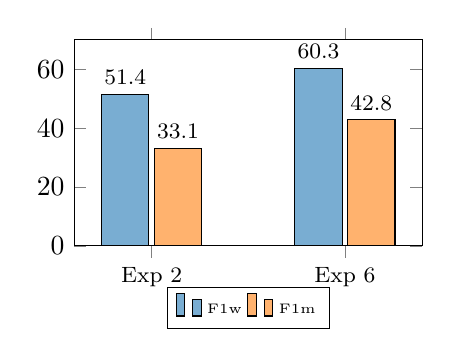
\begin{tikzpicture}
      \begin{axis}[
        width=6cm, height=4.2cm,
        ybar, bar width=0.6cm,
        ymin=0, ymax=70,
        symbolic x coords={Exp 2,Exp 6},
        xtick=data, x tick label style={font=\footnotesize},
        ytick style={font=\footnotesize},
        nodes near coords, nodes near coords style={font=\footnotesize\bfseries},
        enlarge x limits=0.4,
        legend style={font=\tiny, at={(0.5,-0.2)}, anchor=north, legend columns=-1},
      ]
        \addplot[fill=tblue!60] coordinates {(Exp 2,51.4) (Exp 6,60.3)};
        \addlegendentry{F1w}
        \addplot[fill=torange!60] coordinates {(Exp 2,33.1) (Exp 6,42.8)};
        \addlegendentry{F1m}
      \end{axis}
    \end{tikzpicture}
    \footnotesize
    \textbf{+8.9 F1w, +9.7 F1m} \\ (every class improved)
  \end{columns}
\end{frame}

\begin{frame}{Exp 7: Bimodal Ablations --- Who Contributes What?}
  \centering
  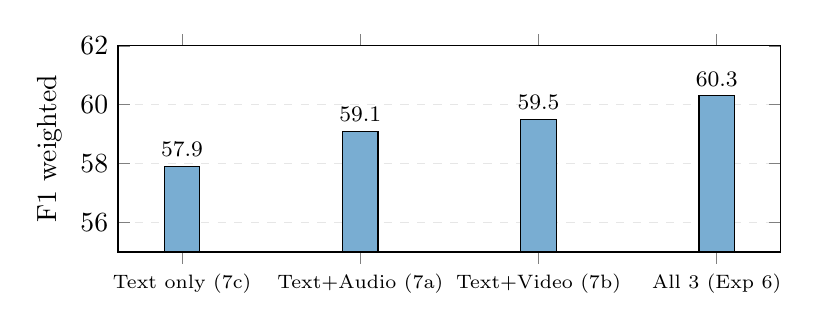
\begin{tikzpicture}
    \begin{axis}[
      width=10cm, height=4.2cm,
      ybar, bar width=0.45cm,
      ylabel={F1 weighted},
      ymin=55, ymax=62,
      symbolic x coords={Text only (7c), Text+Audio (7a), Text+Video (7b), All 3 (Exp 6)},
      xtick=data, x tick label style={font=\scriptsize, align=center},
      ytick style={font=\footnotesize},
      ymajorgrids, grid style={dashed, lightgray},
      nodes near coords, nodes near coords style={font=\footnotesize\bfseries},
      enlarge x limits=0.12,
    ]
      \addplot[fill=tblue!60] coordinates {(Text only (7c),57.9) (Text+Audio (7a),59.1) (Text+Video (7b),59.5) (All 3 (Exp 6),60.3)};
    \end{axis}
  \end{tikzpicture}
  \vfill
  \small
  \begin{itemize}
    \item \textbf{Text alone} = 57.9 F1w --- very close to full 3-modal (60.3)
    \item Audio \& video together add only \textbf{+2.4 F1w} over text
    \item Audio shines on \textbf{Sadness} (prosody); video on \textbf{Neutral} (face grounding)
    \item \emph{Friends} is scripted --- emotion is encoded in word choice
  \end{itemize}
\end{frame}

\begin{frame}{Exp 8: OGM-GE + InfoNCE + Curriculum --- A Wash}
  \begin{columns}[T]
    \column{0.52\textwidth}
    \small
    Three research-backed interventions stacked:
    \vspace{0.2em}
    \begin{enumerate}
      \item \textbf{OGM-GE} (Peng et al., CVPR 2022): rescale weak-branch gradients
      \item \textbf{InfoNCE} (CLIP-style): contrastive alignment across modality pairs
      \item \textbf{Curriculum:} freeze text $\to$ unfreeze $\to$ full
    \end{enumerate}
    \vspace{0.4em}

    \textbf{Result:} F1w $60.3 \to 59.4$ ($-0.9$)
    \vspace{0.3em}

    \textbf{Diagnosis:} Phase A (A+V only) gave \textbf{2\% accuracy} over 3 epochs --- the weak modalities cannot bootstrap alone on MELD.

    \column{0.48\textwidth}
    \centering
    \vspace{0.4em}
    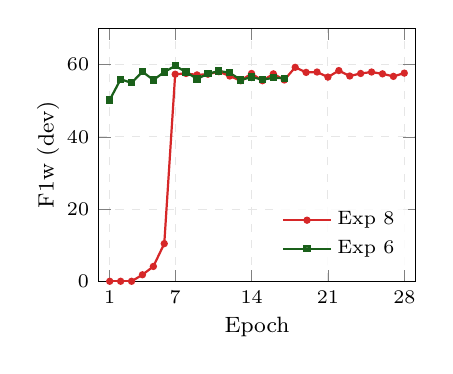
\begin{tikzpicture}
      \begin{axis}[
        width=5.6cm, height=4.8cm,
        xlabel={\footnotesize Epoch},
        ylabel={\footnotesize F1w (dev)},
        xlabel style={yshift=2pt},
        ylabel style={yshift=-4pt},
        ymin=0, ymax=70,
        xmin=0, xmax=29,
        xtick={1,7,14,21,28},
        ytick={0,20,40,60},
        tick label style={font=\scriptsize},
        grid=major, grid style={dashed, lightgray},
        legend style={font=\scriptsize, at={(0.98,0.05)}, anchor=south east, draw=none, fill=white, fill opacity=0.85, text opacity=1},
        every axis plot/.append style={thick},
      ]
        \addplot[tred, mark=*, mark size=0.9pt] coordinates {
          (1,0.1) (2,0.1) (3,0.1) (4,1.9) (5,4.2) (6,10.5) (7,57.3) (8,57.5) (9,57.1) (10,57.3)
          (11,58.0) (12,56.8) (13,55.5) (14,57.5) (15,55.5) (16,57.4) (17,55.7) (18,59.2)
          (19,57.8) (20,57.9) (21,56.5) (22,58.3) (23,56.8) (24,57.5) (25,57.9) (26,57.4) (27,56.7) (28,57.6)
        };
        \addlegendentry{Exp 8}
        \addplot[tgreen!60!black, mark=square*, mark size=0.9pt] coordinates {
          (1,50.2) (2,55.9) (3,54.9) (4,58.0) (5,55.7) (6,57.9) (7,59.6) (8,57.9)
          (9,56.0) (10,57.4) (11,58.2) (12,57.7) (13,55.7) (14,56.5) (15,55.8) (16,56.3) (17,56.2)
        };
        \addlegendentry{Exp 6}
      \end{axis}
    \end{tikzpicture}

    \vspace{0.3em}
    \scriptsize\emph{Phases A \& B are wasted compute.}
  \end{columns}
\end{frame}

\begin{frame}{Exp 9: MHFT Front-End --- The Breakthrough}
  \begin{columns}[t]
    \column{0.55\textwidth}
    \small
    \textbf{Problem:} MultiEMO features are utterance-level (one vector per clip) --- UFEN expects a time sequence.
    \vspace{0.3em}

    \textbf{Solution: MHFT.} Project 1 vector $\to K{=}8$ tokens:
    \[
      \text{MHFT}(x) = \text{reshape}(Wx+b) + P \in \mathbb{R}^{8 \times d_m}
    \]
    UFEN and MTFN run \textbf{unchanged} on the synthetic sequence.
    \vspace{0.3em}

    \textbf{Features:} RoBERTa-768 (T) $+$ openSMILE-512 (A) $+$ DenseNet-1000 (V)

    \column{0.45\textwidth}
    \centering
    \vspace{0.2em}
    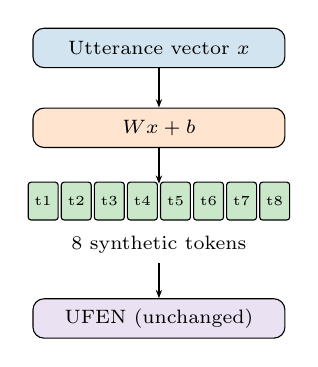
\begin{tikzpicture}[every node/.style={font=\scriptsize},
        box/.style={draw, rounded corners=1pt, minimum width=0.38cm, minimum height=0.48cm, inner sep=0pt, font=\tiny},
        blk/.style={draw, rounded corners, minimum width=3.2cm, minimum height=0.5cm, align=center},
        arr/.style={-{Stealth[length=3pt]}, semithick}]
      \node[blk, fill=tblue!20] (u) {Utterance vector $x$};
      \node[blk, fill=torange!20, below=0.5cm of u] (w) {$Wx + b$};

      % 8 tokens as a horizontal row centered below w
      \node[below=0.55cm of w] (tc) {};
      \foreach \i in {1,...,8} {
        \node[box, fill=tgreen!25] at ($(tc) + (0.42*\i - 1.89, 0)$) (t\i) {t\i};
      }
      \node[font=\scriptsize] at ($(tc) + (0, -0.55)$) (tlabel) {8 synthetic tokens};

      \node[blk, fill=tpurple!20, below=0.45cm of tlabel] (ufen) {UFEN (unchanged)};

      \draw[arr] (u) -- (w);
      \draw[arr] (w.south) -- ($(tc) + (0, 0.22)$);
      \draw[arr] (tlabel.south) -- (ufen.north);
    \end{tikzpicture}

    \vspace{0.5em}
    \scriptsize\textbf{F1w: 60.3 $\to$ 61.5}\\[0.15em]
    \textbf{Params: 111M $\to$ 3.58M} (\textbf{30$\times$ shrink})
  \end{columns}
\end{frame}

\begin{frame}{Exp 9.1: Closing the Dev$\to$Test Gap}
  \small
  \textbf{Problem:} Exp 9 had dev F1w = 71.7 but test = 61.5 --- a \textbf{10-point} generalisation gap.
  \vspace{0.3em}

  \textbf{Root cause:} Random split of \texttt{trainVid} leaked \emph{Friends} speakers into dev. Model memorised speaker-specific patterns.
  \vspace{0.5em}

  \textbf{Three fixes:}
  \begin{columns}[t]
    \column{0.33\textwidth}
    \centering
    \textbf{1. Speaker-disjoint split}\\[0.3em]
    \footnotesize Hold out whole dialogue groups by dominant speaker
    \vspace{0.3em}\\
    \tiny Gap: $10.2 \to 5.7$

    \column{0.33\textwidth}
    \centering
    \textbf{2. Capped class weights}\\[0.3em]
    \footnotesize Cap Fear/Disgust weights at 1.5 (was 2.24 / 2.41)
    \vspace{0.3em}\\
    \tiny False positives: $84 \to 43$

    \column{0.33\textwidth}
    \centering
    \textbf{3. Top-5 ensemble}\\[0.3em]
    \footnotesize Average softmax of top-5 dev checkpoints
    \vspace{0.3em}\\
    \tiny $+0.9$ F1m free
  \end{columns}
  \vfill
  \centering
  \begin{tabular}{lccc}
    \toprule
    & \textbf{Exp 9} & \textbf{Exp 9.1} & \textbf{$\Delta$} \\
    \midrule
    Test F1w   & 61.5 & \textbf{64.4} & +2.9 \\
    Test F1m   & 45.7 & \textbf{49.0} & +3.3 \\
    Train size & 9{,}920 & 6{,}464 & $-3{,}456$ \\
    \bottomrule
  \end{tabular}
  \vspace{0.3em}\\
  \footnotesize \emph{Less training data, better generalisation.}
\end{frame}

% ============================================================
\section{Analysis}
% ============================================================

\begin{frame}{Per-Class F1 --- Exp 9.1 vs.\ Baselines}
  \centering
  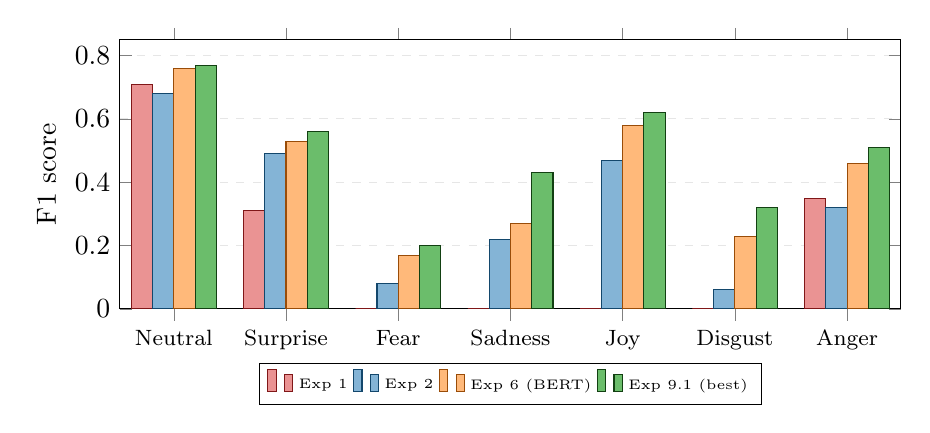
\begin{tikzpicture}
    \begin{axis}[
      width=11.5cm, height=5cm,
      ybar=0pt, bar width=0.27cm,
      ymin=0, ymax=0.85,
      ylabel={F1 score},
      symbolic x coords={Neutral,Surprise,Fear,Sadness,Joy,Disgust,Anger},
      xtick=data, x tick label style={font=\footnotesize},
      ytick style={font=\footnotesize},
      ymajorgrids, grid style={dashed, lightgray},
      legend style={font=\tiny, at={(0.5,-0.2)}, anchor=north, legend columns=-1},
      enlarge x limits=0.08,
    ]
      \addplot[fill=tred!50, draw=tred!60!black] coordinates {
        (Neutral,0.71) (Surprise,0.31) (Fear,0.00) (Sadness,0.00)
        (Joy,0.00) (Disgust,0.00) (Anger,0.35)
      };
      \addlegendentry{Exp 1}
      \addplot[fill=tblue!55, draw=tblue!60!black] coordinates {
        (Neutral,0.68) (Surprise,0.49) (Fear,0.08) (Sadness,0.22)
        (Joy,0.47) (Disgust,0.06) (Anger,0.32)
      };
      \addlegendentry{Exp 2}
      \addplot[fill=torange!55, draw=torange!60!black] coordinates {
        (Neutral,0.76) (Surprise,0.53) (Fear,0.17) (Sadness,0.27)
        (Joy,0.58) (Disgust,0.23) (Anger,0.46)
      };
      \addlegendentry{Exp 6 (BERT)}
      \addplot[fill=tgreen!70, draw=tgreen!40!black] coordinates {
        (Neutral,0.77) (Surprise,0.56) (Fear,0.20) (Sadness,0.43)
        (Joy,0.62) (Disgust,0.32) (Anger,0.51)
      };
      \addlegendentry{Exp 9.1 (best)}
    \end{axis}
  \end{tikzpicture}
  \vfill
  \footnotesize
  Exp 9.1 wins or ties on \textbf{5/7 classes}. Largest gains: Sadness ($+0.08$), Disgust ($+0.07$), Anger ($+0.04$).
\end{frame}

\begin{frame}{What Did \emph{Not} Help --- and Why}
  \small
  \begin{tabular}{p{4.5cm}p{2cm}p{6cm}}
    \toprule
    \textbf{Attempted} & \textbf{$\Delta$ F1w} & \textbf{Root cause} \\
    \midrule
    Focal loss ($\gamma = 2$) & $-0.9$ & Over-penalises easy Neutral/Joy, hurts mid-frequency classes \\
    Video projection 2048$\to$256 & $-1.1$ & BiGRU implicitly selects channels end-to-end; fixed projection discards \\
    Doubled capacity ($d_m=256$) & $-1.1$ & 7.1M params on 10K samples $\to$ instability (best ep = 3) \\
    Lower LR ($5{\times}10^{-4}$) & $-1.1$ & Slower convergence, no better final \\
    Scheduled unfreezing & $-0.9$ & A/V cannot bootstrap alone (2\% accuracy in Phase A) \\
    \bottomrule
  \end{tabular}
  \vfill
  \centering
  \textbf{Lesson:} on small datasets with one dominant modality, small surgical fixes beat elaborate interventions.
\end{frame}

\begin{frame}{Error Analysis --- Exp 9.1 Confusion Patterns}
  \begin{columns}[T]
    \column{0.42\textwidth}
    \small
    \vspace{0.5em}
    Three persistent patterns:
    \vspace{0.4em}
    \begin{enumerate}
      \item \textbf{Neutral absorbs errors} --- $\sim$7--10\% of every other class pulled into Neutral
      \item \textbf{Anger/Surprise/Joy triangle} --- shared high-arousal prosody
      \item \textbf{Fear \& Disgust} still hard (50 \& 68 test samples)
    \end{enumerate}

    \column{0.58\textwidth}
    \centering
    \vspace{0.3em}
    \scriptsize
    \setlength{\tabcolsep}{3pt}
    \renewcommand{\arraystretch}{1.15}
    \begin{tabular}{l ccccccc}
      \toprule
               & \textbf{Neu} & \textbf{Sur} & \textbf{Fear} & \textbf{Sad} & \textbf{Joy} & \textbf{Dis} & \textbf{Ang} \\
      \midrule
      Neutral  & \cellcolor{tgreen!45}\textbf{912} & 65 & 43 & 60 & 84 & 28 & 64 \\
      Surprise & 24 & \cellcolor{tgreen!45}\textbf{177} & 4 & 4 & 27 & 10 & 35 \\
      Fear     & 9 & 4 & \cellcolor{torange!45}\textbf{17} & 6 & 5 & 1 & 8 \\
      Sadness  & 40 & 14 & 26 & \cellcolor{torange!45}\textbf{83} & 12 & 6 & 27 \\
      Joy      & 59 & 40 & 8 & 6 & \cellcolor{tgreen!45}\textbf{253} & 10 & 26 \\
      Disgust  & 14 & 5 & 4 & 2 & 0 & \cellcolor{torange!45}\textbf{28} & 15 \\
      Anger    & 44 & 41 & 17 & 13 & 29 & 22 & \cellcolor{tgreen!45}\textbf{179} \\
      \bottomrule
    \end{tabular}
    \vspace{0.4em}

    \tiny \emph{Diagonal = correct predictions; green = strong, orange = weak.}
  \end{columns}
\end{frame}

% ============================================================
\section{Wrapping Up}
% ============================================================

\begin{frame}{Key Takeaways}
  \small
  \begin{enumerate}
    \item \textbf{UFEN+MTFN architecture is sound} --- every component is ablation-justified on MOSI.
    \item \textbf{BERT is the dominant lever on MELD:} context-free embeddings plateau at $\sim$51 F1w; fine-tuned BERT jumps it to 60.3.
    \item \textbf{MHFT is the surprise winner:} 3.58M params beats 111M BERT on every MELD metric. Pre-extracted features + a lightweight tokenization bridge is a very favourable trade.
    \item \textbf{Evaluation integrity matters as much as architecture:} swapping a random dev split for speaker-disjoint closed a 4-point gap with \emph{less} training data.
    \item \textbf{Negative results are informative:} focal loss, doubled capacity, and curriculum unfreezing all failed --- each teaches something about the dataset.
  \end{enumerate}
\end{frame}

\begin{frame}{Limitations \& Future Work}
  \begin{columns}[t]
    \column{0.5\textwidth}
    \textbf{Limitations}
    \begin{itemize}
      \item Small datasets (MOSI: 1.3K; MELD: 10K train)
      \item Single-seed reporting (no std)
      \item Paper hyperparameters under-specified
      \item Wave2Vec2-32 \& ResNet-101 are not SOTA for affect
      \item No inter-utterance context
    \end{itemize}

    \column{0.5\textwidth}
    \textbf{Future Work}
    \begin{itemize}
      \item Multi-seed mean $\pm$ std
      \item Stronger A/V extractors: \\ WavLM, Whisper, AffectNet
      \item Dialogue context (DialogueRNN-style)
      \item MHFT on time-aligned features
      \item Extend to MOSEI, IEMOCAP, CH-SIMS
    \end{itemize}
  \end{columns}
  \vfill
  \footnotesize
  \textbf{Ethical note:} MELD is drawn from \emph{Friends}, a US sitcom with a narrow demographic and scripted emotion. Deployed systems need re-validation on diverse populations and spontaneous speech.
\end{frame}

\begin{frame}[standout]
  \begin{center}
    \huge Thank you!\\[1em]
    \normalsize Questions?\\[2em]
    \small
    \textbf{Code:} \url{github.com/Gautam-Gandhi/multimodal-sentiment-analysis}\\[0.5em]
    \textbf{Team TokeNization:} Manas, Soham, Parth, Gautam
  \end{center}
\end{frame}

\end{document}
